% vim: textwidth=80
\documentclass{article}

% packages
\usepackage[pdftex]{graphicx}
\usepackage{listings}
\usepackage{float}

% set the code to wrap and have box
\lstset{
    frame=single,
    breaklines=true
}

% set the graphics path
\graphicspath{ {./plots/} }

\begin{document}

\title{CS 199 BD Homework 3}
\author{Jay Bensal, Richard Lee, Raj Ramamurthy\\
  NetIDs: bensal2, rlee46, rlee46}

% Title
\maketitle

% You should build a linear regression of violent crimes per population against
% explanatory variables that don't have missing values. Check your regression ---
% are there problem data points? which ones, and why? Does a Box-Cox
% transformation make things better?
\section{Linear Regression}
Upon building a linear regression, we noticed that
there are a lot of data points which were missing values. In order to build our
linear regression, we removed these values.

\section{Sample plot}
% figure with H flag (put it here)
\begin{figure}[H]
\centering
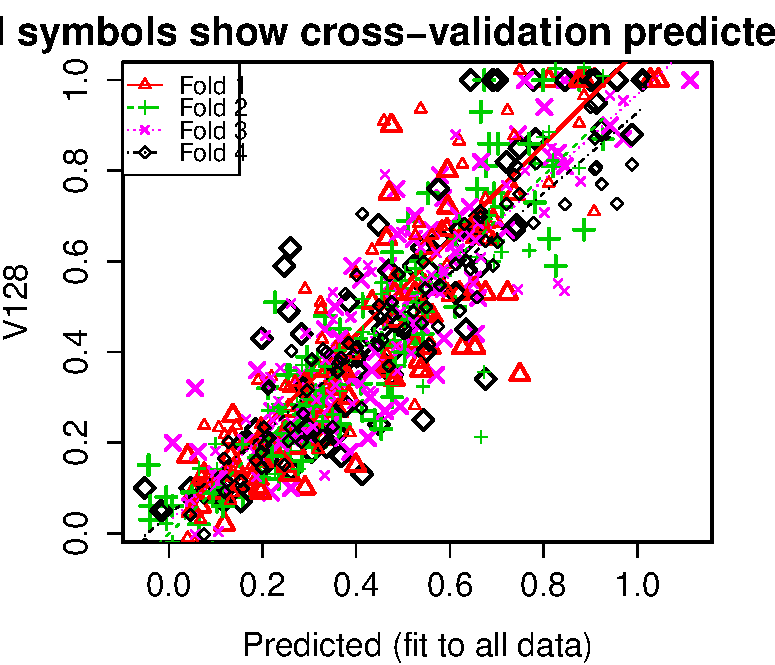
\includegraphics[width=3.0in]{part1a.pdf}
\caption{Plot one}\label{fig_container} 
\end{figure}

\section{R Code}
\begin{lstlisting}[language=r]
crime<-read.csv('communities.data', header=FALSE)
crime<-crime[c(-1,-2,-3,-4,-5)]
crime<-crime[sample(nrow(crime)),]
crime[crime == '?'] <- NA
#replace all '?' with NA
drop_cols <- crime[complete.cases(crime), ] # only take the variables w/ all the values
library(DAAG)
fit<-lm(V128 ~ V6+ V7+ V8+ V9+ V10+ V11+ V12+ V13+ V14+ V15+ V16+ V17+ V18+ V19+ V20+ V21+ V22+ V23+ V24+ V25+ V26+ V27+ V28+ V29+ V30+ V32+ V33+ V34+ V35+ V36+ V37+ V38+ V39+ V40+ V41+ V42+ V43+ V44+ V45+ V46+ V47+ V48+ V49+ V50+ V51+ V52+ V53+ V54+ V55+ V56+ V57+ V58+ V59+ V60+ V61+ V62+ V63+ V64+ V65+ V66+ V67+ V68+ V69+ V70+ V71+ V72+ V73+ V74+ V75+ V76+ V77+ V78+ V79+ V80+ V81+ V82+ V83+ V84+ V85+ V86+ V87+ V88+ V89+ V90+ V91+ V92+ V93+ V94+ V95+ V96+ V97+ V98+ V99+ V100+ V101+ V119+ V120+ V121+ V126, data=drop_cols)
cv.lm(df=drop_cols, fit, m=4)
library('MASS')
boxcox(fit, lambda = seq(0, 1, 1/10), plotit=TRUE)
crime_lambda1 = drop_cols
for (i in 1:nrow(crime_lambda1)){
  crime_lambda1[i, ncol(crime_lambda1)] = (crime_lambda1[i, ncol(crime_lambda1)]^0.3-1)/0.3
}

fit2<-lm(V128 ~ V6+ V7+ V8+ V9+ V10+ V11+ V12+ V13+ V14+ V15+ V16+ V17+ V18+ V19+ V20+ V21+ V22+ V23+ V24+ V25+ V26+ V27+ V28+ V29+ V30+ V32+ V33+ V34+ V35+ V36+ V37+ V38+ V39+ V40+ V41+ V42+ V43+ V44+ V45+ V46+ V47+ V48+ V49+ V50+ V51+ V52+ V53+ V54+ V55+ V56+ V57+ V58+ V59+ V60+ V61+ V62+ V63+ V64+ V65+ V66+ V67+ V68+ V69+ V70+ V71+ V72+ V73+ V74+ V75+ V76+ V77+ V78+ V79+ V80+ V81+ V82+ V83+ V84+ V85+ V86+ V87+ V88+ V89+ V90+ V91+ V92+ V93+ V94+ V95+ V96+ V97+ V98+ V99+ V100+ V101+ V119+ V120+ V121+ V126, data=crime_lambda1)
cv.lm(df=crime_lambda1, fit2, m=4)

################## KNN ####################################

comm<-read.csv('communities.data', header=FALSE);
comm<-comm[c(-1,-2,-3,-4,-5)] 
#delete the first 5 vars which are not predictive

library('FNN')
#comm = comm[sample(nrow(comm)),]
comm[comm == '?'] <- NA
#replace all '?' with NA
full <- comm[complete.cases(comm),]
#then only take the ones w/ all the values
lapply(full, as.numeric)

full = subset(full, select=-c(V31, V102, V103, V104, V105, V106, V107, V108, V109, V111, V110, V112, V113, V114, V115, V116, V117, V118, V122, V123, V124, V125, V127))
comm_full = subset(comm, select=-c(V31, V102, V103, V104, V105, V106, V107, V108, V109, V111, V110, V112, V113, V114, V115, V116, V117, V118, V122, V123, V124, V125, V127))
#do some nearest neighbor stuff
wtrain <- full[1:100,1:(ncol(full)-1)]
wtrl <- full[1:100,(ncol(full))]
wtest <- full[101:200, 1:(ncol(full)-1)]
wtel <- full[101:200, ncol(full)]
#results = knn(wtrain, wtest, wtrl, k = 10, algorithm="cover_tree")
results = knn(wtrain, wtest, wtrl, k = 21, algorithm="cover_tree")
plot(as.numeric(results), as.numeric(wtel))
library(impute)
imputed=impute.knn(as.matrix(comm_full), k=10)
fit<-lm(V128 ~ V6+ V7+ V8+ V9+ V10+ V11+ V12+ V13+ V14+ V15+ V16+ V17+ V18+ V19+ V20+ V21+ V22+ V23+ V24+ V25+ V26+ V27+ V28+ V29+ V30+ V32+ V33+ V34+ V35+ V36+ V37+ V38+ V39+ V40+ V41+ V42+ V43+ V44+ V45+ V46+ V47+ V48+ V49+ V50+ V51+ V52+ V53+ V54+ V55+ V56+ V57+ V58+ V59+ V60+ V61+ V62+ V63+ V64+ V65+ V66+ V67+ V68+ V69+ V70+ V71+ V72+ V73+ V74+ V75+ V76+ V77+ V78+ V79+ V80+ V81+ V82+ V83+ V84+ V85+ V86+ V87+ V88+ V89+ V90+ V91+ V92+ V93+ V94+ V95+ V96+ V97+ V98+ V99+ V100+ V101+ V119+ V120+ V121+ V126, data=as.data.frame(imputed$data))
cv.lm(df=as.data.frame(imputed$data), fit, m=4)
\end{lstlisting}

\end{document}
